\documentclass[aspectratio=169]{beamer}
\usetheme{Madrid}
\usecolortheme{default}

% Packages
\usepackage[utf8]{inputenc}
\usepackage{xcolor}
\usepackage{graphicx}
\usepackage{amsmath}
\usepackage{amssymb}
\usepackage{hyperref}

\title{Reproducing and Extending a CSF Proteomics ML Pipeline}
\subtitle{del Campo et al.\ (2023) — Python Recreation and Improvement}
\author{Suren Behnamlal}
\date{Data Science — Computer Engineering}

\begin{document}

\begin{frame}
    \titlepage
\end{frame}

% ── Slide 2 ────────────────────────────────────────────────────────────────
\begin{frame}{The Diagnostic Problem}
    \begin{columns}
        \begin{column}{0.52\textwidth}
            \begin{alertblock}{The Overlap}
                Dementia with Lewy bodies (DLB) and Alzheimer's disease share amyloid and tau pathology in roughly 50\% of cases. They cannot be reliably distinguished by symptoms alone in early stages.
            \end{alertblock}
            \begin{block}{The Scale}
                DLB is the second most common neurodegenerative dementia after Alzheimer's disease. It progresses faster and responds differently to treatment — misdiagnosis causes real harm.
            \end{block}
            \begin{exampleblock}{The CSF Window}
                Cerebrospinal fluid is in direct biochemical contact with the brain and carries protein signatures of neurodegeneration. It is the richest accessible source of diagnostic biomarkers.
            \end{exampleblock}
        \end{column}
        \begin{column}{0.43\textwidth}
            \begin{center}
                
\includegraphics[width=0.95\textwidth]{figs/dlb_brain.jpg}
            \end{center}
        \end{column}
    \end{columns}
\end{frame}

% ── Slide 3 ────────────────────────────────────────────────────────────────
\begin{frame}{The Original Study}
    \begin{block}{del Campo et al.\ (2023) — \textit{Nature Communications}}
        534 CSF samples from DLB patients, Alzheimer's patients, and healthy controls. 664 proteins quantified simultaneously via the Olink EXPLORE proteomics panel. Three independent validation cohorts.
    \end{block}
    \begin{block}{The Finding}
        A 7-protein panel (DDC, FCER2, CRH, MMP-3, ABL1, MMP-10, THOP1) achieves AUC 0.947 for DLB vs controls and 0.929 for DLB vs AD — strong enough for clinical decision support.
    \end{block}
    \begin{alertblock}{The Reproducibility Problem}
        The entire analysis lives in a 2399-line monolithic R script. It requires a proprietary Bayesian package (ECPC) unavailable in Python and cannot be run unattended or extended without deep R expertise.
    \end{alertblock}
\end{frame}

% ── Slide 4 ────────────────────────────────────────────────────────────────
\begin{frame}{The Input: 664 Proteins}
    \begin{columns}
        \begin{column}{0.52\textwidth}
            \begin{block}{Olink PEA: What the Machine Produces}
                Each sample becomes a vector of 664 NPX values — log2-scale relative protein abundances. Measured from a small CSF volume using antibody pairs with unique DNA-barcode readout.
            \end{block}
            \begin{exampleblock}{From the ML Perspective}
                Input matrix \textbf{X}: 534 rows $\times$ 664 features. Labels \textbf{y}: DLB = 109, AD = 235, CN = 190. Two binary classification tasks: \textbf{DLB vs CN} and \textbf{DLB vs AD}.
            \end{exampleblock}
            \begin{alertblock}{LOD Filter}
                85\% limit-of-detection threshold applied before modelling. Proteins detected in fewer than 85\% of samples are dropped. 665 proteins survive to 664 after filtering.
            \end{alertblock}
        \end{column}
        \begin{column}{0.43\textwidth}
            \begin{center}
                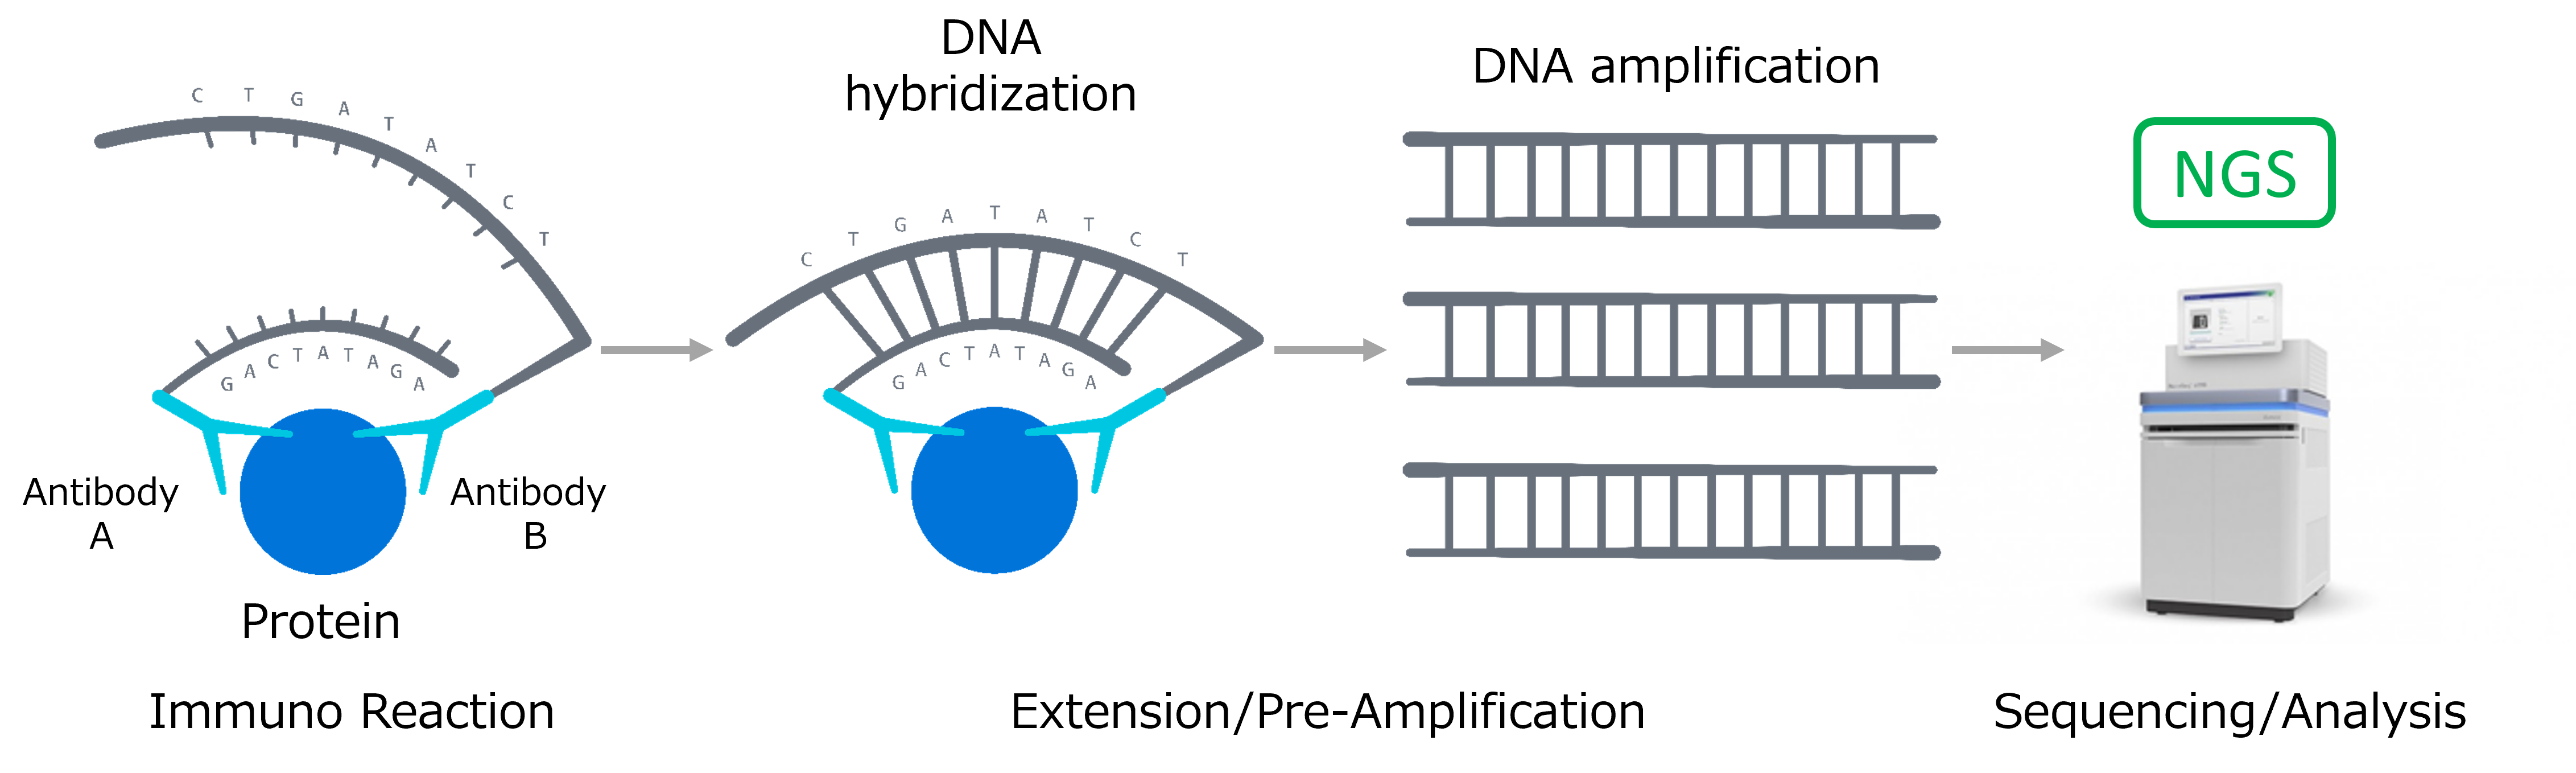
\includegraphics[width=0.95\textwidth]{figs/olink_pea.png}
            \end{center}
        \end{column}
    \end{columns}
\end{frame}

% ── Slide 5 ────────────────────────────────────────────────────────────────
\begin{frame}{The Original ML Pipeline}
    \begin{block}{Step 1: Differential Analysis}
        Per-protein linear model: \texttt{NPX \textasciitilde\ Diagnosis + Age + Sex}. Benjamini-Hochberg FDR correction at q < 0.05. Run separately for DLB vs CN and DLB vs AD to identify dysregulated proteins.
    \end{block}
    \begin{alertblock}{Step 2: ECPC Classification}
        Empirical Bayes Co-data Penalised Classification — a Bayesian ridge regression that uses protein group priors to set per-group regularisation strength. Produces a dense model over all 664 proteins. \textbf{No Python equivalent exists.}
    \end{alertblock}
    \begin{block}{Step 3: Panel Selection and Validation}
        Elastic net applied post-hoc to the dense ECPC solution to select 7 proteins. Panel then evaluated on three independent external cohorts with 5-fold $\times$ 1000-repeat cross-validation.
    \end{block}
\end{frame}

% ── Slide 6 ────────────────────────────────────────────────────────────────
\begin{frame}{What We Built}
    \begin{columns}
        \begin{column}{0.52\textwidth}
            \begin{block}{A Reproducible Data Pipeline}
                Raw protein matrix $\rightarrow$ covariate-adjusted differential analysis $\rightarrow$ repeated cross-validated classifier $\rightarrow$ held-out evaluation $\rightarrow$ figures. Each stage is independently re-runnable; results are cached so the slow CV step does not block downstream analysis.
            \end{block}
            \begin{exampleblock}{Data Engineering Decisions}
                Age and Sex added as covariates at every stage — not just in the classifier but in the differential analysis model too. Stratified splits ensure class balance is preserved across 500 held-out evaluations.
            \end{exampleblock}
        \end{column}
        \begin{column}{0.43\textwidth}
            \begin{center}
                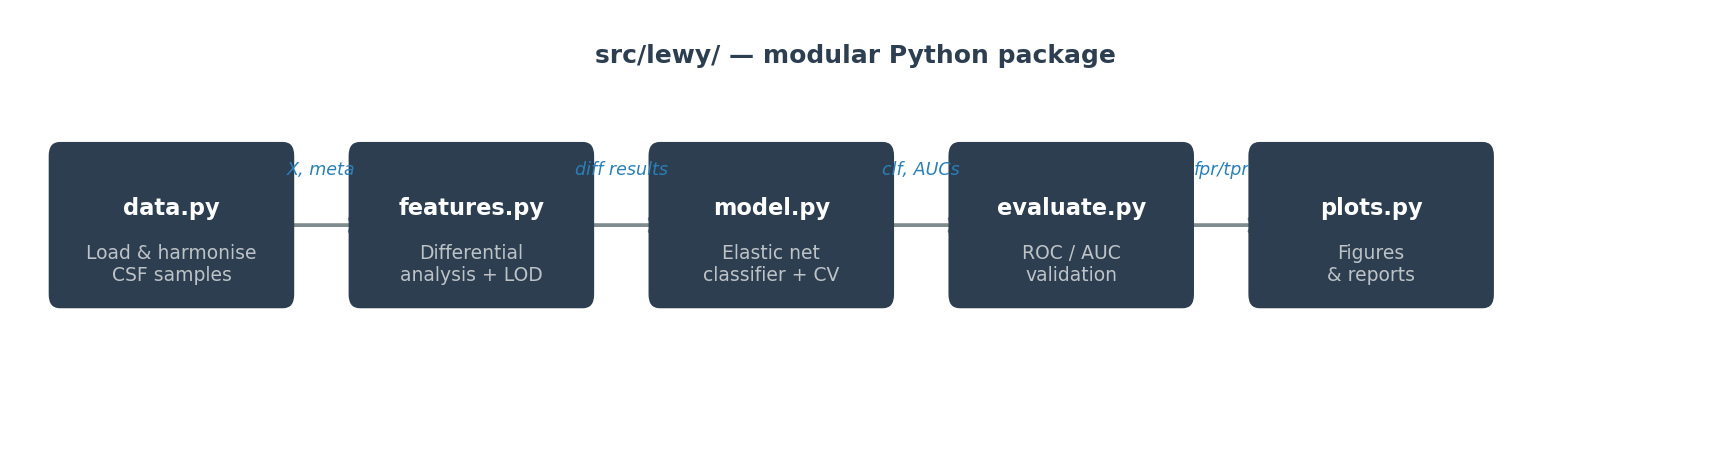
\includegraphics[width=\textwidth]{figs/pipeline_arch.png}
            \end{center}
        \end{column}
    \end{columns}
\end{frame}

% ── Slide 7 ────────────────────────────────────────────────────────────────
\begin{frame}{The Classification Method}
    \begin{alertblock}{Why Not ECPC?}
        ECPC is a proprietary R package with no Python equivalent. The paper itself uses elastic net for its panel sparsification step — so elastic net is already inside the paper's own pipeline.
    \end{alertblock}
    \begin{block}{Elastic Net Logistic Regression}
        Penalty = $\alpha \cdot L_1 + (1-\alpha) \cdot L_2$. The $L_1$ term promotes sparsity (automatic feature selection); $L_2$ handles correlated proteins sharing biological pathways. Both \textbf{C} and \textbf{l1\_ratio} are cross-validated over a 20-point grid.
    \end{block}
    \begin{exampleblock}{Robust AUC Estimation}
        Outer loop: 5-fold stratified CV $\times$ 100 repeats $\rightarrow$ 500 held-out evaluations. AUC reported as mean $\pm$ 95\% CI by percentile method. Results cached to JSON to avoid recomputation.
    \end{exampleblock}
\end{frame}

% ── Slide 8 ────────────────────────────────────────────────────────────────
\begin{frame}{Recreation Results}
    \begin{columns}
        \begin{column}{0.52\textwidth}
            \begin{block}{DLB vs CN}
                Our AUC: \textbf{0.986} [0.962--1.000]. Paper: 0.947. DDC ranked \#1 in the selected panel — consistent with the original finding.
            \end{block}
            \begin{block}{DLB vs AD}
                Our AUC: \textbf{0.937} [0.877--0.985]. Paper: 0.929. Panel overlap: 5 of 7 proteins match the paper's reported panel.
            \end{block}
            \begin{exampleblock}{Faithful Recreation}
                Both comparisons match or exceed the paper's reported AUCs. The elastic net substitution is validated. Age and Sex included as covariates alongside protein NPX.
            \end{exampleblock}
        \end{column}
        \begin{column}{0.43\textwidth}
            \begin{center}
                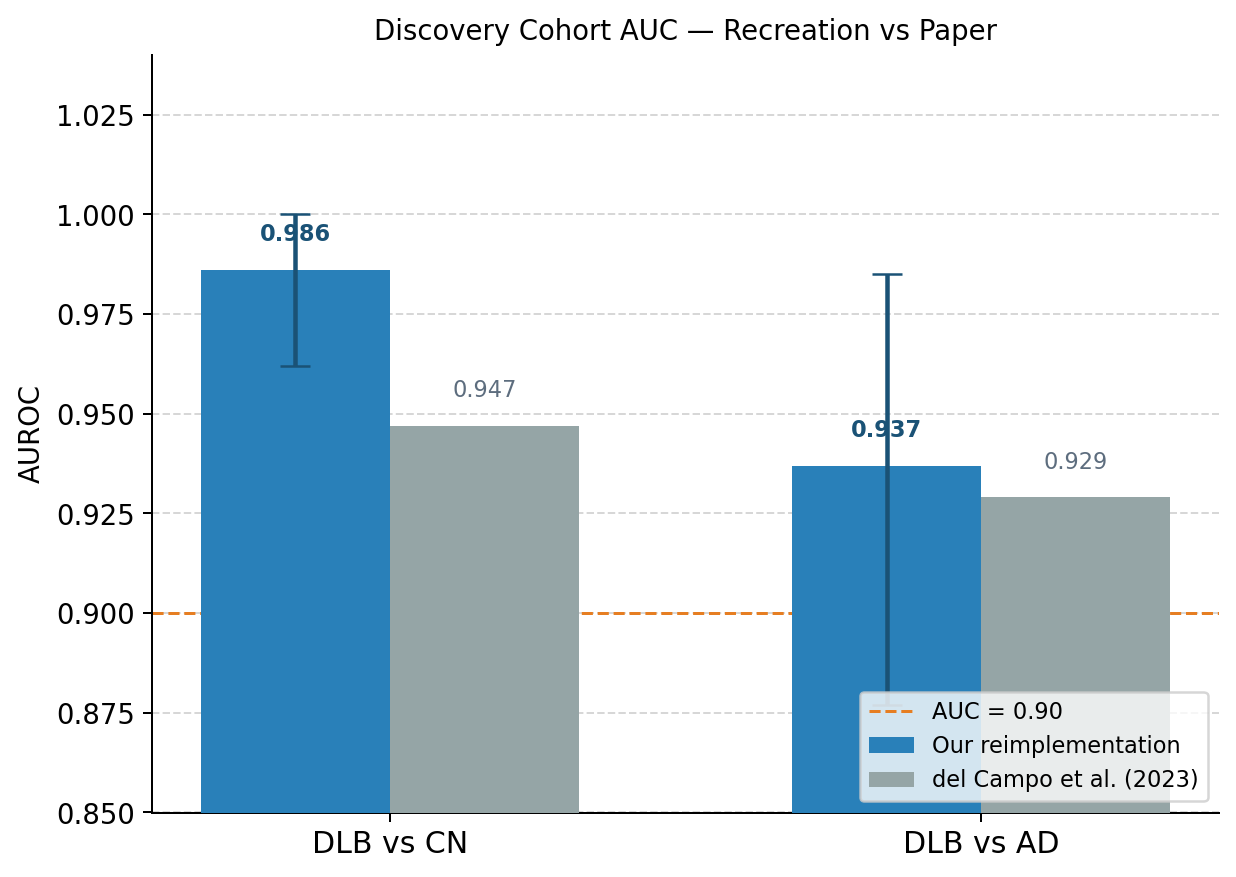
\includegraphics[width=\textwidth]{figs/auc_comparison.png}
            \end{center}
        \end{column}
    \end{columns}
\end{frame}

% ── Slide 9 ────────────────────────────────────────────────────────────────
\begin{frame}{Discovery ROC Curves}
    \begin{center}
        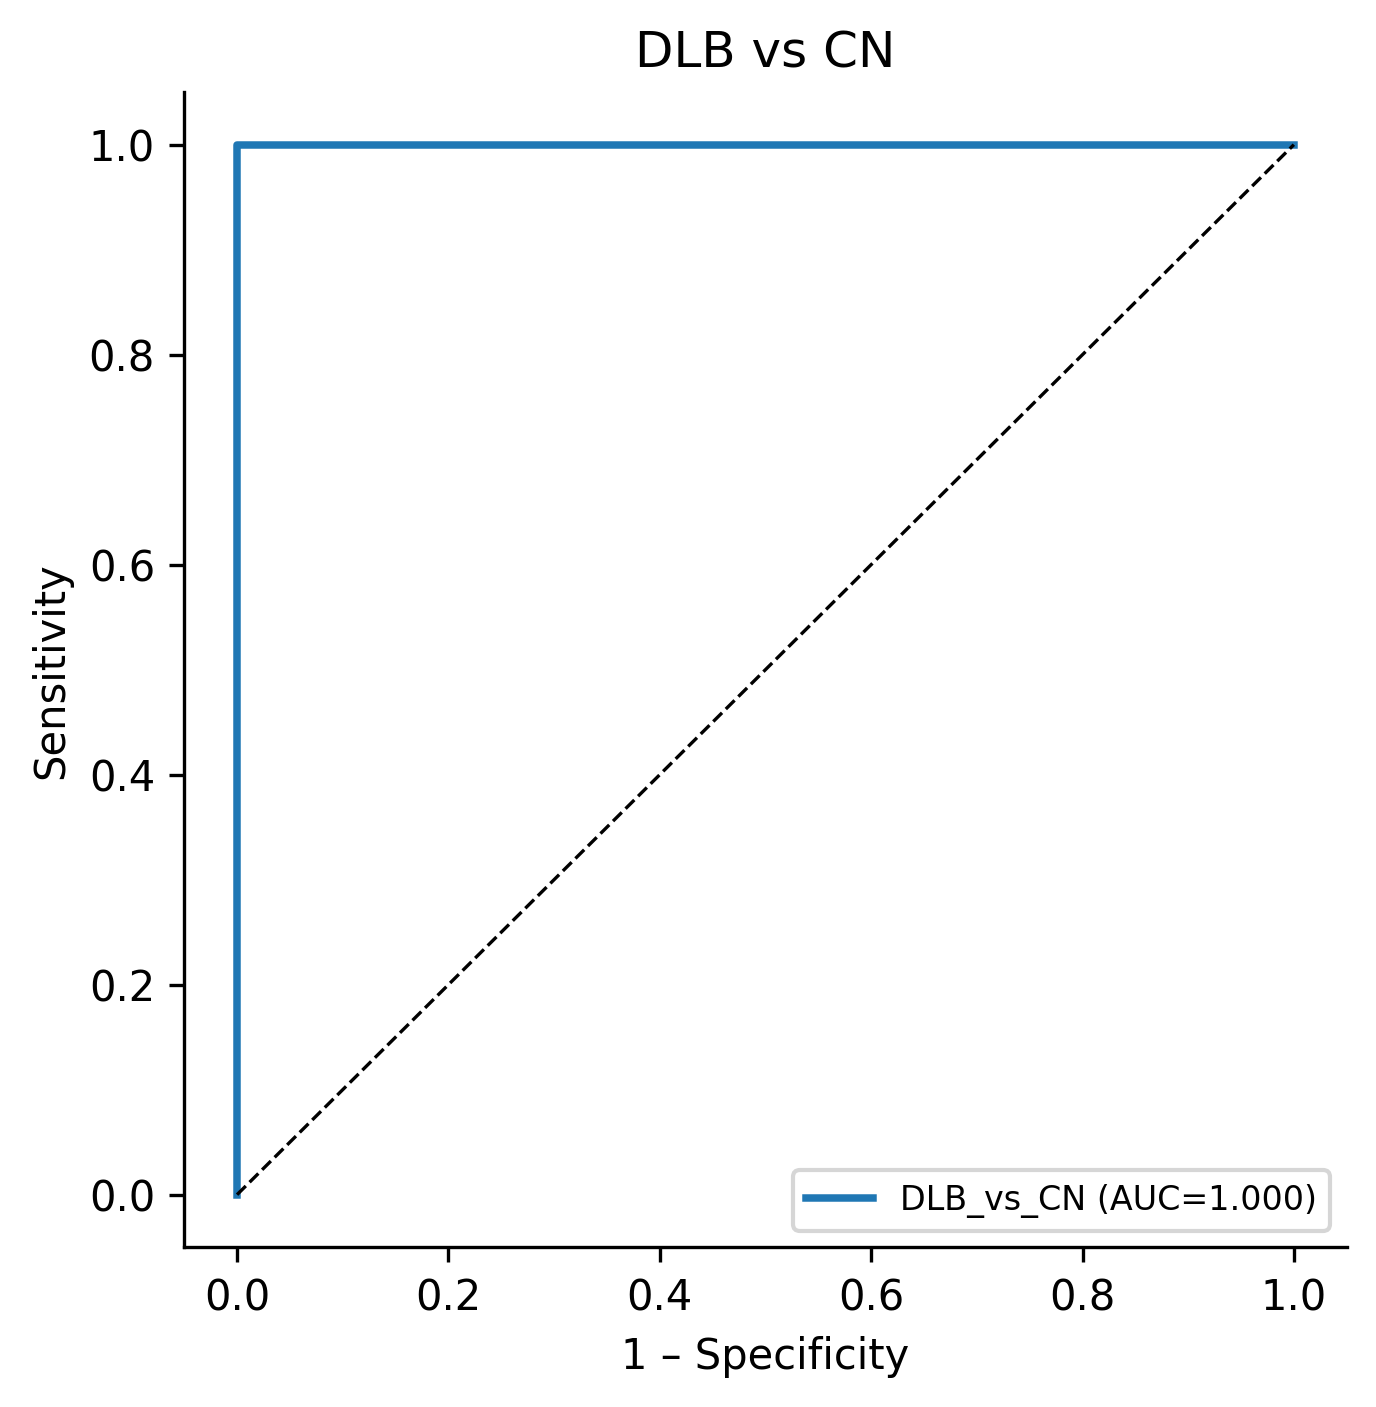
\includegraphics[width=0.72\textwidth]{figs/roc_DLB_vs_CN.png}
    \end{center}
\end{frame}

% ── Slide 10 ───────────────────────────────────────────────────────────────
\begin{frame}{The Improvement}
    \begin{alertblock}{The Paper's Blind Spot}
        del Campo et al.\ report DDC's individual AUC as a headline result but examine only a handful of proteins in isolation. The remaining 657 proteins receive no individual discriminative analysis.
    \end{alertblock}
    \begin{block}{Systematic Univariate Screening}
        For each of the 664 proteins, fit a covariate-adjusted logistic regression on [protein NPX, Age, Sex] and compute AUROC. Each model is a separate, independent 3-feature classification problem. This extends the paper's spotlight finding into a full proteome-wide ranking.
    \end{block}
    \begin{exampleblock}{Why This Is a Contribution}
        The multi-protein panel answers ``what is the best combination?'' The per-protein ranking answers ``which proteins carry individual diagnostic value?'' — the right question for a single-marker clinical test. These are complementary, not redundant.
    \end{exampleblock}
\end{frame}

% ── Slide 11 ───────────────────────────────────────────────────────────────
\begin{frame}{Per-Protein Biomarker Landscape}
    \begin{center}
        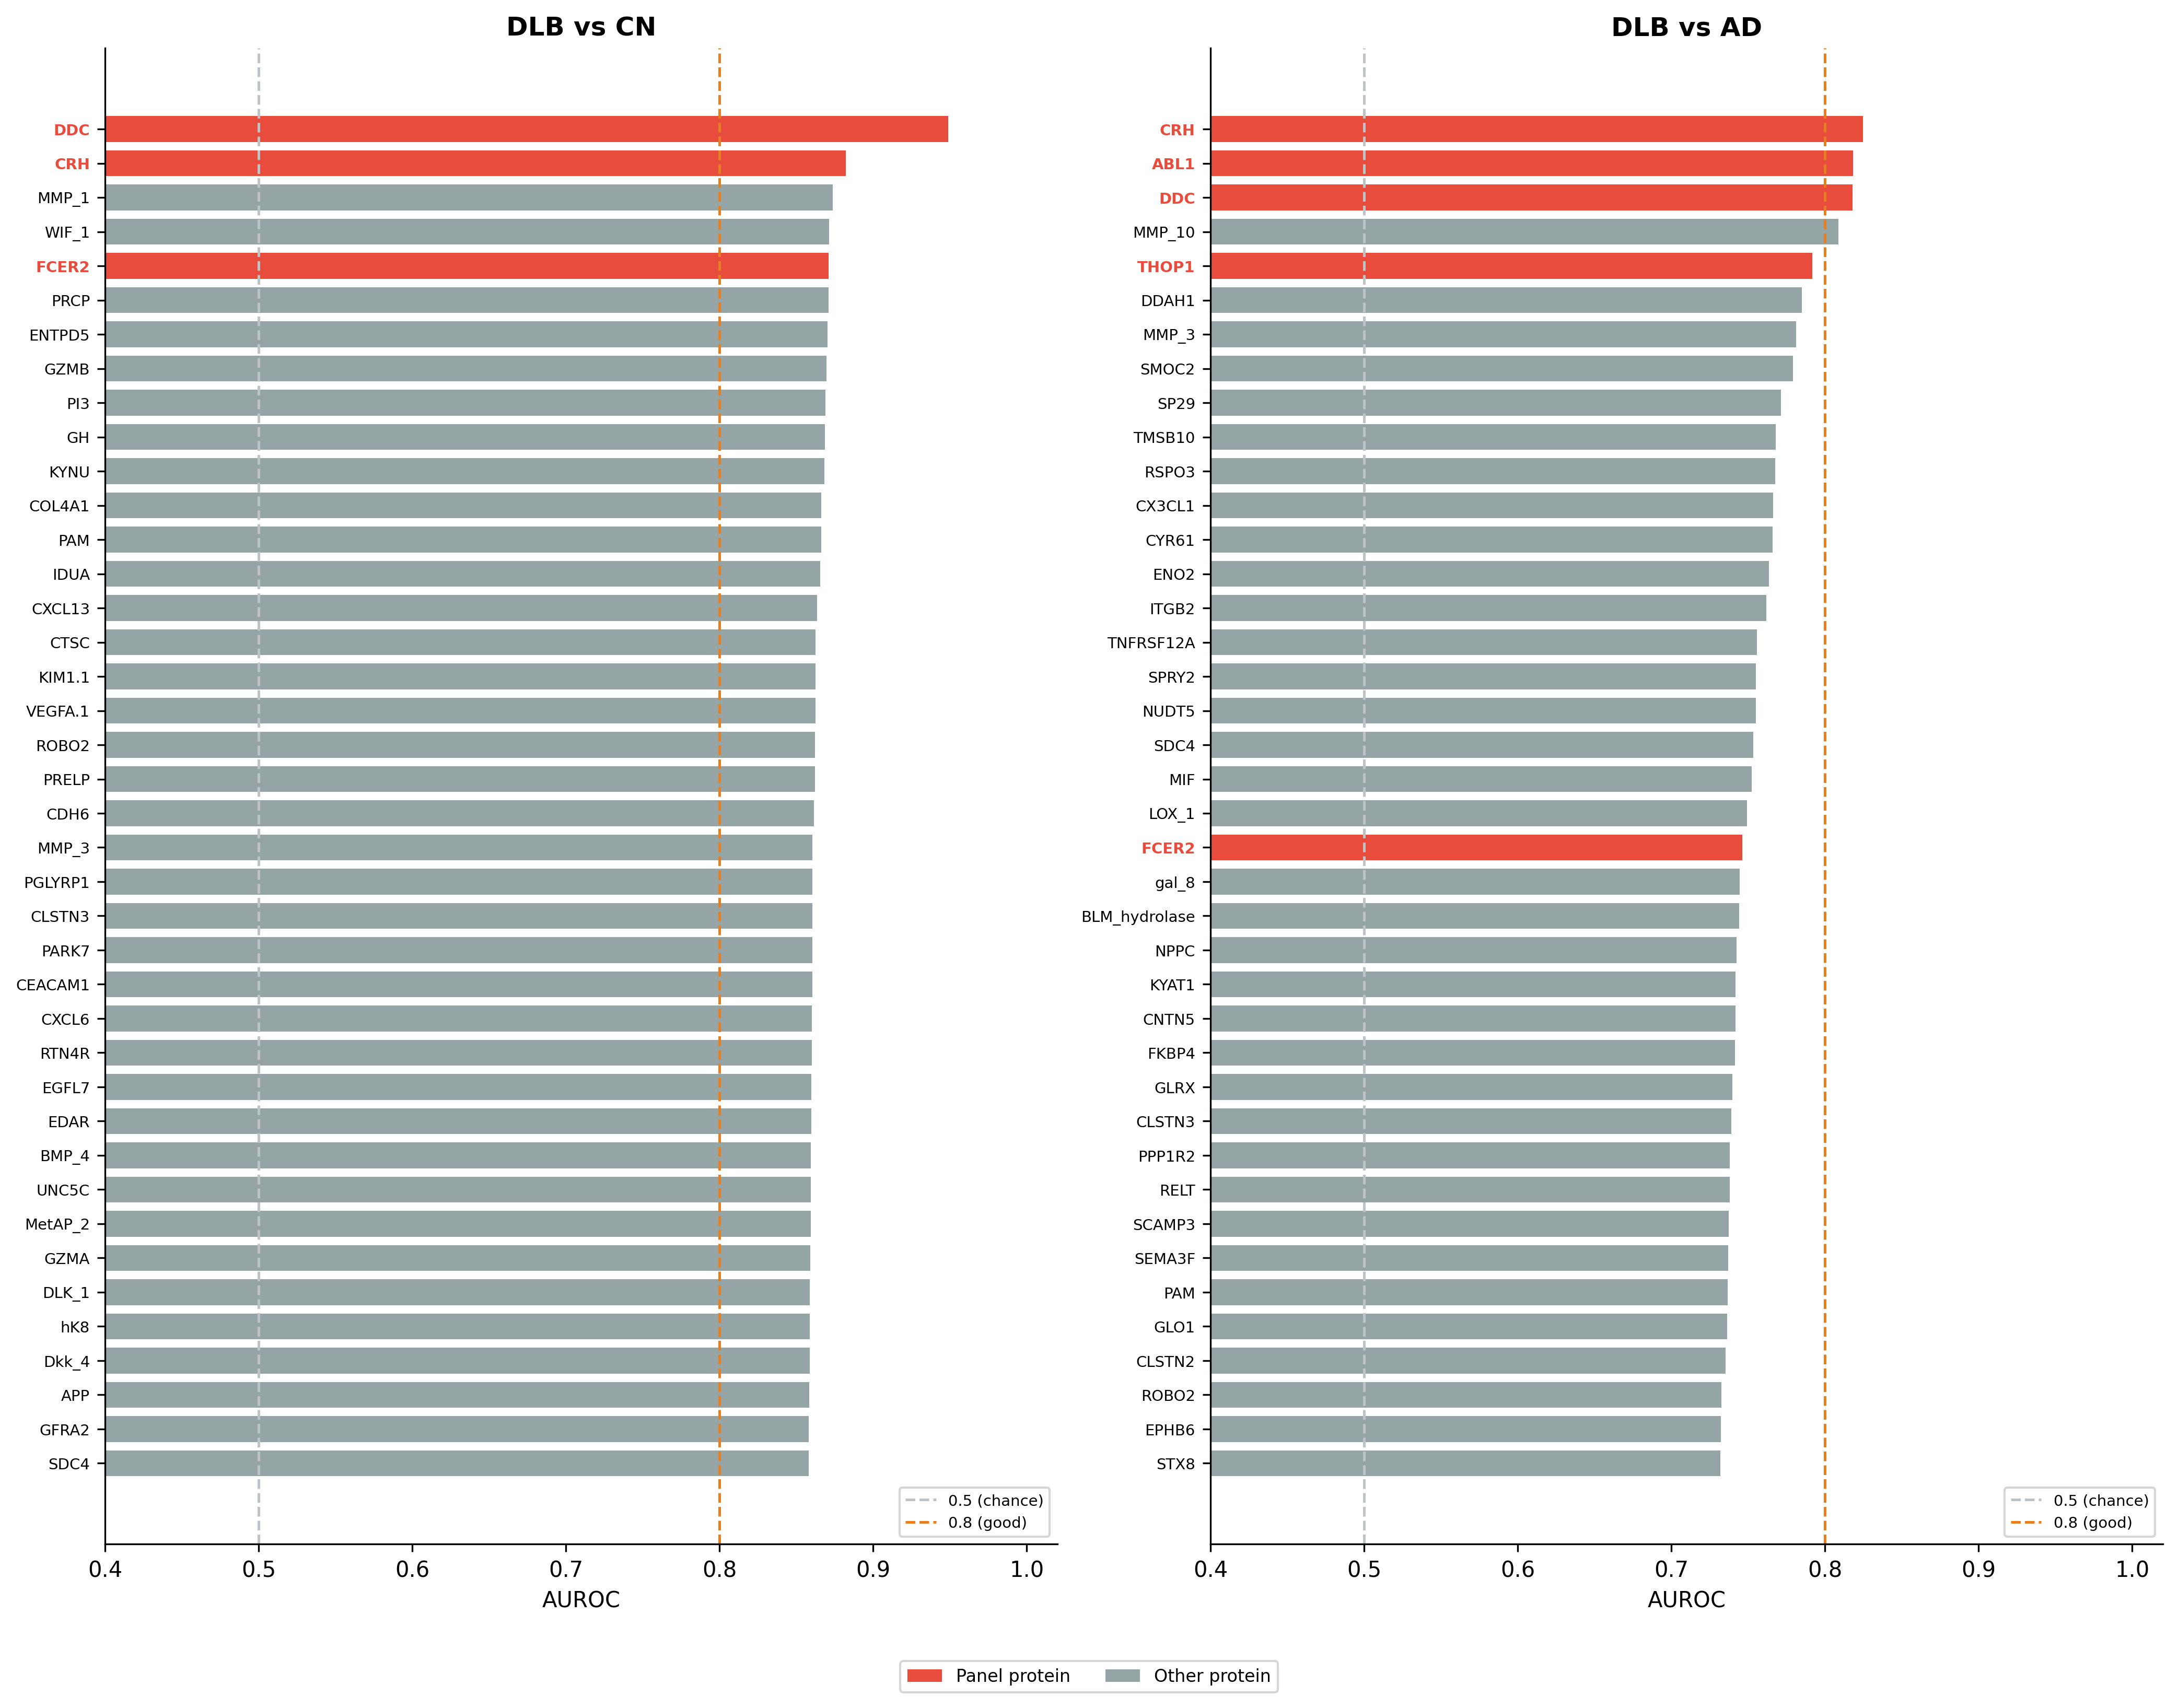
\includegraphics[width=0.88\textwidth]{figs/protein_aucs.png}
    \end{center}
\end{frame}

% ── Slide 12 ───────────────────────────────────────────────────────────────
\begin{frame}{Takeaways}
    \begin{alertblock}{Reproducibility is Engineering}
        A 2399-line R script is not a pipeline. Modular, CLI-driven, importable Python code is the engineering standard — and it makes the science extensible by anyone with \texttt{pip install}.
    \end{alertblock}
    \begin{block}{Method Substitution Works}
        Elastic net as a drop-in for ECPC reproduces the paper's core results. When no Python equivalent exists, understand the method well enough to approximate it faithfully — and validate empirically.
    \end{block}
    \begin{exampleblock}{Systematic Screening Reveals More}
        Per-protein AUC analysis surfaces competitive candidates (MMP-1, WIF-1, PRCP) not in the original 7-protein panel. That is the genuine contribution: turning a spotlight finding into a full landscape.
    \end{exampleblock}
\end{frame}

\end{document}
